% Created 2017-07-24 Mon 21:42
% Intended LaTeX compiler: pdflatex
\documentclass[journal=jacsat,manuscript=suppinfo,email=true,hyperref=true,keywords=true]{achemso}
 \usepackage{minted}
 \usepackage{graphicx}
\usepackage{float}
\usepackage{xcolor}
\usepackage{amsmath}
\usepackage{fontspec}
\author{Tian Tian}
\affiliation{Institute for Chemical and Bioengineering, ETH Z{\"{u}}rich,  Vladimir Prelog Weg 1, CH-8093 Z{\"{u}}rich, Switzerland}
\author{Shangchao Lin}
\email{slin@eng.fsu.edu.}
\affiliation{Department of Mechanical Engineering, Materials Science and Engineering Program, FAMU-FSU College of Engineering, Florida State University, Tallahassee, Florida 32310, United States}
\author{Siyu Li}
\affiliation{Key Laboratory of Energy Thermal Conversion and Control of Ministry of Education, School of Energy and Environment, Southeast University, Nanjing, Jiangsu 210096, China}
\author{Lingling Zhao}
\affiliation{Key Laboratory of Energy Thermal Conversion and Control of Ministry of Education, School of Energy and Environment, Southeast University, Nanjing, Jiangsu 210096, China}
\author{Elton J. G. Santos}
\affiliation{School of Mathematics and Physics, Queen's University Belfast, United Kingdom, BT7 1NN, United Kingdom}
\author{Chih-Jen Shih}
\email{chih-jen.shih@chem.ethz.ch}
\affiliation{Institute for Chemical and Bioengineering, ETH Z{\"{u}}rich,  Vladimir Prelog Weg 1, CH-8093 Z{\"{u}}rich, Switzerland}
\date{}
\title{Doping-Driven Wettability of Two-Dimensional Materials: a Multiscale Theory}
\begin{document}

\newpage{}
\section{Figures}
\label{sec:orgedeb1ea}
\subsection{Dipole Orientation Profiles of MD Simulations}
\label{sec:org0dfc0ff}
\begin{figure}[htbp]
\centering
\includegraphics[width=0.85\linewidth]{../img/SI-dipole-profile.pdf}
\caption{\label{fig-SI-dipole}
Dipole orientation \(\cos \mu\) as a function of \(z\) in MD simulations of different systems (L, and GL with varied graphene doping densities). The orientation at the water-vacuum interface (\(z=20\) nm) is invariable in all cases, indicating a minimal effect of the long range Coulombic interaction on the selected interface.}
\end{figure}

\newpage{}

\subsection{Properties of First Water Layer Adjacent to Charged Graphene Surface}
\label{sec:org697bf5c}
\begin{figure}[htbp]
\centering
\includegraphics[width=.9\linewidth]{../img/SI_prop_1st_layer.pdf}
\caption{\label{fig-SI-1st}
Properties of the first water layer adjacent to the charged graphene surface. The following quantities are plotted as a function of \(\sigma_{\mathrm{2D}}\): (a) z-position of the first water layer with maximal value of \(\rho_{\mathrm{L}}\). (b) maximal \(\rho_{\mathrm{L}}\) of the first water layer. (c) z-position of the first water layer with maximal value of \(\delta_{\mathrm{L}}\). and (d) maximal \(\delta_{\mathrm{L}}\) of the first water layer.}
\end{figure}
\newpage{}


\subsection{Hydrogen Bond Profiles of MD Simulations}
\label{sec:orgd29efcb}

\begin{figure}[htbp]
\centering
\includegraphics[width=0.85\linewidth]{../img/hydrogen-bond.pdf}
\caption{\label{fig-H-bond}
Hydrogen bond density (\(\rho_{\mathrm{HB}}\)) as a function of \(z\) in MD simulations of various conditions (L, GL with graphene doping densities of -0.012, 0 and 0.012  \textit{e}/atom).}
\end{figure}

\newpage{}


\subsection{Explanation for Shift of \(\Delta \Phi_{\mathrm{Coul}}\) Maximum from Charge Neutral State}
\label{sec:orgdeeca1e}

As can be seen in Figure 3(c) in the main text, the maximum of \(\Delta
\Phi_{\mathrm{Coul}}\) as function of \(\sigma_{\mathrm{2D}}\) shifts
from charge neutral state (\(\sigma_{\mathrm{2D}} = 0\)) to slightly
n-doped region. This behavior can be explained by the contribution
from the interfacial charge density to the Coulombic interactions (Figure \ref{fig-SI-mode}(a)).
Assuming that the interfacial charge density per unit area of the
water layer \(\sigma_{\mathrm{L}}\) is approximated by
\(\sigma_{\mathrm{L}}=\delta_{\mathrm{L}} \cdot t_{1}\), where \(t_{1}\)
is the thickness of the 1st water layer (\textasciitilde{}2.8 \AA{}). The interfacial
Coulombic potential caused by the 1st charged layer is then:
\begin{equation}
\label{eq:1}
\begin{aligned}
\Phi_{\mathrm{Coul}}^{\mathrm{int}} &= \frac{\sigma_{\mathrm{2D}} \sigma_{\mathrm{L}}}{2C_{\mathrm{int}}} \\
                                           &= \frac{\sigma_{\mathrm{2D}} \delta_{\mathrm{L}} t_{1} d_{1}}{2\epsilon_{\mathrm{int}}}
\end{aligned}
\end{equation}
where \(C_{\mathrm{int}}=\epsilon_{\mathrm{int}}/d_{1}\) is the
geometric capacitance of the interfacial void, \(\epsilon_{1}\) and
\(d_{1}\) are the permittivity and thickness of the interfacial void. We
assume that the interfacial dielectric constant
\(\epsilon_{\mathrm{int}} = 20 \epsilon_{0}\)
\cite{conway_dielectric_1951}, and take the value of \(d_{1}\) from the
value of the most probable charge distribution distance \(z_{1}\) from
Figure \ref{fig-SI-1st}(c). The comparison between the \(\Delta
\Phi_{\mathrm{Coul}}\) from MD results and the proposed model can be
seen in Figure \ref{fig-SI-mode}(b). The degree of Coulombic
interactions from the model is close to that of the MD results,
indicating that the decrease of interaction potential of the
graphene-water system is mainly determined by the interfacial charge
distribution. The result predicted by the model also shows a shifted
maximum of \(\Delta \Phi_{\mathrm{Coul}}\), well corresponding with the
MD results. Such asymmetric behavior is further ascribed to the
decrease of \(\delta_{\mathrm{L}}\) when graphene is slightly n-doped
(see Figure \ref{fig-SI-1st}(d)), as a combined result of the Coulombic
interaction and hydrogen bonding. Note that in the p-doped regime, the
model-predicted \(\Delta \Phi_{\mathrm{Coul}}\) value differs from the
MD results, suggesting that the contribution from the subsequent
layers are important.

\begin{figure}[htbp]
\centering
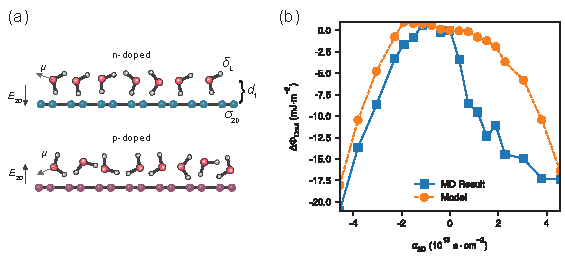
\includegraphics[width=0.95\linewidth]{../img/SI_model.pdf}
\caption{\label{fig-SI-mode}
Simple model for the asymmetric behavior of \(\Delta \Phi_{\mathrm{Coul}}\) as a function of \(\sigma_{\mathrm{2D}}\). (a) Proposed orientation of first layer water molecules on n- and p-doped graphene surface. (b) Comparison between the \(\Delta \Phi_{\mathrm{Coul}}\) values calculated by MD simulation and the proposed model. The results obtained by the simple capacitance model shows similar shift of \(\Delta \Phi_{\mathrm{2D}}\) maximum.}
\end{figure}


\clearpage{}

\subsection{Fitting of the \(\Delta \Phi\) - \(\sigma_{\mathrm{2D}}\) Data in MD Simulations}
\label{sec:org7e59573}


\begin{figure}[htbp]
\centering
\includegraphics[width=0.85\linewidth]{../img/e-Phi_vdw-fitting.pdf}
\caption{\label{fig-SI-fitting}
Best fitting  results of \(\Delta \Phi_{\mathrm{LJ}}\) and \(\Delta \Phi_{\mathrm{Coul}}\) as functions of \(\sigma_{\mathrm{2D}}\) for n- and p-doped graphene-water systems. Total potential change \(\Delta \Phi\) is fitted by combining the fitting results of LJ and Coulombic potentials}
\end{figure}

\newpage{}


\bibliography{ref}
\end{document}